%%Introduction

In this Section, we consider models with a photon, a W boson, a Z boson or a Higgs boson in the final state, 
accompanied by Dark Matter particles that either couple directly to the boson or are mediated by 
a new particle. The experimental signature is identified as \textit{V+MET}. 

These models are interesting both as extensions of models where the gluon provides 
the experimentally detectable signature, 
and as stand-alone models with final states that cannot be generated by the models in
Section~\ref{subsec:MonojetLikeModels}.

%%%Classification of models

\begin{figure}[h!]
  \centering
    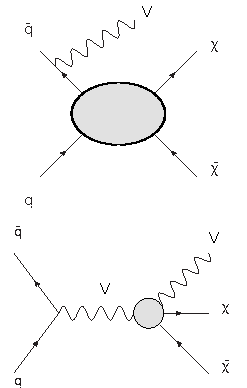
\includegraphics[width=0.5\textwidth]{figures/EW/VPlusMET_EFT}
  \caption{Sketch of benchmark models including a contact interaction 
  for V+MET searches, adapted from~\cite{Nelson:2013pqa}. \label{fig:VPlusMET_EFT}}
\end{figure}
% 
The models considered can be divided in categories:
\begin{description}
 \item[Models including a contact operator, where the boson is radiated from the initial state] As depicted in 
 the top diagram of Figure~\ref{fig:VPlusMET_EFT}, these models follow the nomenclature and theory 
 for the EFT benchmarks commonly used by MET+X searches~\cite{Goodman:2010ku}. These models
 have been used in past experimental searches~~\cite{Khachatryan:2014rwa, Aad:2014vka,Khachatryan:2014tva, Aad:2014vka, 
 ATLAS:2014wra, Aad:2013oja}, and they will not be described here. 
 \item[Models including a contact operator, where the boson is directly coupled to DM]
 Shown in the bottom of Figure~\ref{fig:VPlusMET_EFT},
 these models allow for a contact interaction vertex that directly couples the boson to Dark Matter. 
 \item[Simplified models where the boson is radiated from the initial state] These models follow those
 already described in Section~\ref{subsec:MonojetLikeModels}, replacing the initial state gluon with a boson.
 \item[V-specific simplified models] These models postulate direct couplings of new mediators
 to bosons, e.g. they couple the Higgs boson to a new scalar~\cite{Carpenter:2013xra}. 
\end{description}

The following Sections describe the models within these categories, 
the parameters for each of the benchmark models chosen,
the studies towards the choices of the parameters to be scanned, 
and finally point to the location of their Matrix Element 
implementation. 

\newthought{Simplified models with ISR boson radiation}

Searches in the jet+MET final state are generally more sensitive
with respect to final states including bosons, due to the much 
larger rates of signal events featuring quark or gluon radiation with 
respect to radiation of bosons~\cite{Zhou:2013fla}, 
in combination with the low branching ratios if leptons from 
boson decays are required in the final state. 
The rates for the Higgs boson radiation is too low for these models 
to be considered a viable benchmark~\cite{Carpenter:2013xra}.
However, the presence of photons
leptons from W and Z decays
and W or Z bosons decaying hadronically
allows to reject the background more effectively, making Z/gamma/W+MET searches 
still worth comparing with searches in the jet+MET final state. 

% The three commonly chosen EFT benchmarks for Dirac dark matter that are 
% kinematically distinct for what concerns the observables used in 
% MET+X searches~\footnote{[CD: we would need a plot here, or a reference to 
% monojet section where this is shown]} and span a wide range of MET spectrum in 
% the boson+MET searches are, in the notation of ~\cite{Goodman:2010ku}, 
% the D1 (scalar SM/WIMP interaction), D5 (vector-vector interaction) and D9 
% (tensor interaction) operator. 

\paragraph{Vector mediator exchanged in the s-channel}

The case for searches with W bosons in the final state has so far been strenghtened by the 
presence of particular choices of couplings between the WIMP and the up and 
down quarks which enhance W radiation~\cite{Bai:2012xg}, in the case of the exchange
of a vector mediator in the s-channel. 
Run-1 searches have considered three sample cases for the product of 
up and down quark couplings to the mediator $\xi$:
\begin{itemize}
 \item No couplings between mediator and either up or down quarks~($\xi=0$);
 \item Same coupling between mediator and each of the quark types~ ($\xi=1$);
 \item Coupling of opposite sign between mediator and each of the quark types~($\xi=-1$). 
\end{itemize}
The $\xi=-1$ case leads to a large increase in the cross-section of the process,
and modifies the spectrum of missing transverse energy or 
transverse mass used for the searches. The sensitivity of the W+MET search for 
this benchmark in this case surpasses that of the jet+MET search. 
However, as shown in Ref.~\cite{Bell:2015sza}, the cross-section increase is due
to the production of longitudinally polarized W bosons, 
as a consequence of a violation of electroweak gauge symmetries. Unless further
particles are introduced (in a fashion similar
to the Higgs boson in the Standard Model), choosing a value of $\xi=-1$ 
for this simplified model will lead to a manifest violation of unitarity at LHC energies. 
The simplified model with a vector mediator exchanged in the s-channel model 
can still be considered as a benchmark for searches with a W boson if $\xi=1$. 
We leave the study of further models with cross-section enhancements due
to different couplings to up and down quarks for studies beyond the early LHC searches
covered in this document. 
\textbf{[TODO: Substitute the following sentence with Yang Bai's paragraph]}. 
An example of such model is the case of both DM and SM Higgs charged under a new U(1)',
with a a small mass mixing between SM Z-boson and the new Zprime. This leads
to different effective DM couplings to $u_L$ and $d_L$, proportional to
their coupling to the Z boson. 

The scan in the parameters that characterize of this model follow what
already detailed in Section~\ref{subsec:MonojetLikeModels}. 
%FIXME: refer to appropriate subsection

% CD: I tend to like this list so I'll leave it here in hope of recycling it
% \begin{itemize}
%  \item the mass of the DM particle ($m_{DM}$);
%  \item the mediator mass ($m_{Med}$);
%  \item the mediator width ($\Gamma_{Med}$);
%  \item the couplings between the DM and the mediator ($g_{DM}$), 
%  and between the mediator and the initial state quarks ($g_{SM}$);
%  \item the chirality of the couplings between DM and mediator, 
%  and between mediator and initial state quarks (vector-vector, axial-vector, axial-axial, vector-axial).
% \end{itemize}

As in the case of the jet+MET models, the width does not have a significant
impact on the kinematic distributions relevant for those searches. An example
of the particle-level analysis acceptance using the
generator-level cuts from Ref.~\cite{Aad:2014tda} 
for the photon+MET analysis, but raising the photon $p_T$ cut
to 150 GeV is shown in Figure~\ref{fig:DMV_EW_gamma_acceptance}, 
comparing a width that is set to $\Gamma=M_{med}/3$ to the
minimal width (the ratio between the two widths 
ranges from 1.05 to 1.5 with increasing mediator masses).

% mMed : minW
% 10  : 3.5
% 50 : 21.3
% 100 : 42.4
% 300 : 127.3
% 600 : 300.1
% 1000 : 503
% 3000 : 1512
% 6000 : 3024

\begin{figure}
    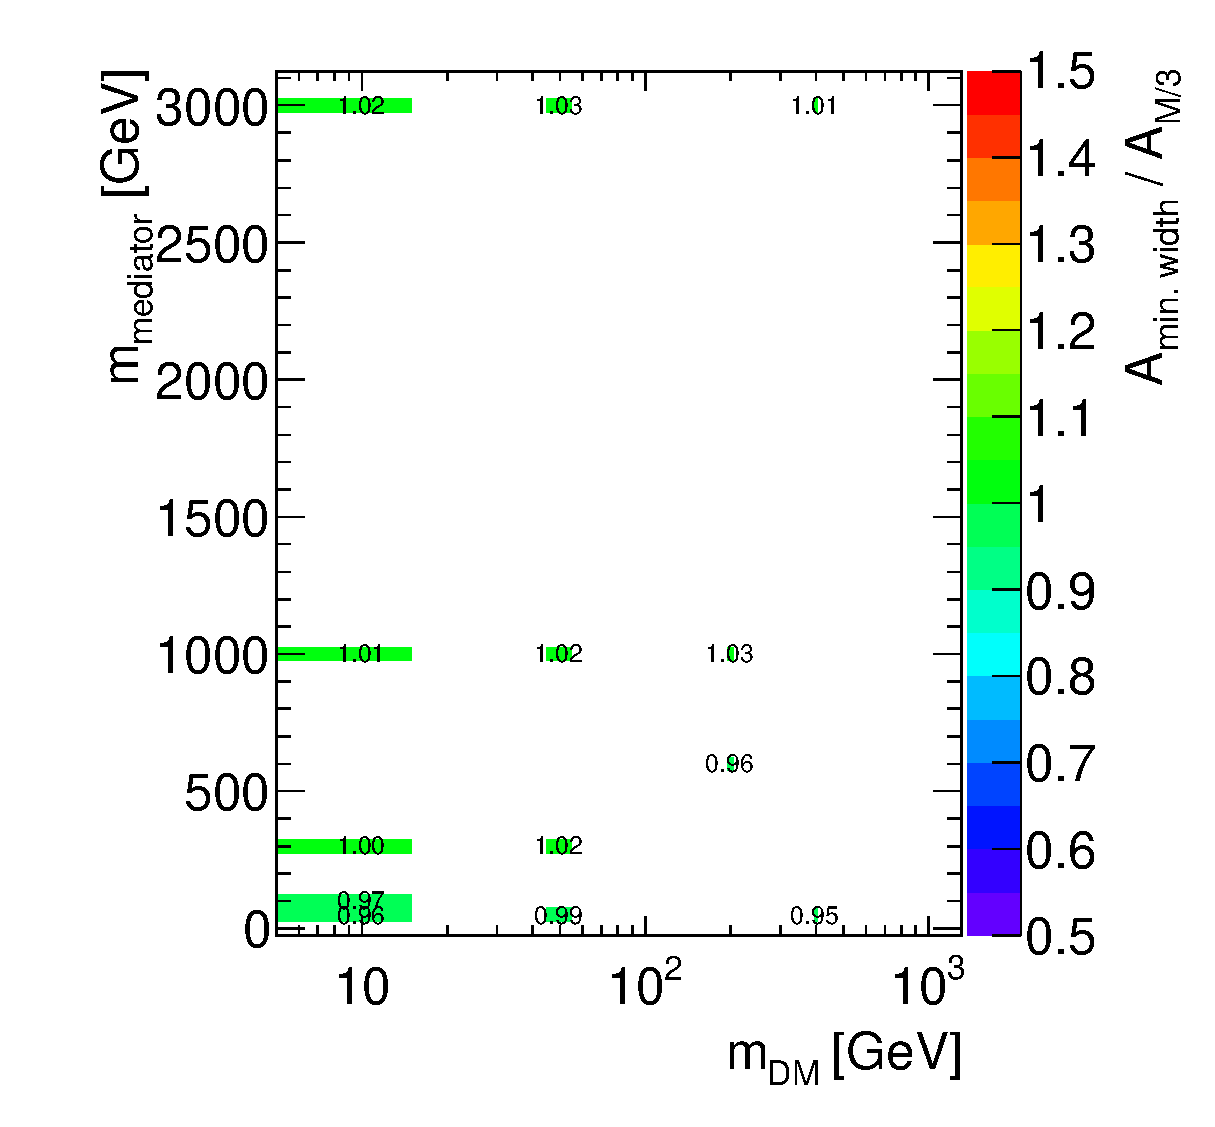
\includegraphics[width=0.7\textwidth]{figures/EW/acceptance_minwidth_vs_mo3_gamma}
    \caption{Analysis acceptance for the photon+MET analysis when varying the mediator width, in the
    case of a vector mediator exchanged in the $s-$channel}%This plot will come from Marie-Helene
    \label{fig:DMV_EW_gamma_acceptance}
\end{figure}

Examples of relevant kinematic distributions for selected benchmark points are
shown in Fig.~\ref{fig:DMV_EW_kinematics}; leading-order cross-sections for the chosen 
benchmark points are shown in Table~\ref{table:x-sec}
\textbf{[TODO: Insert table of cross-sections]}.

\begin{figure}[h!]
  \centering  
  \subfloat[Missing transverse momentum distribution for the photon+MET final state, for 
  different mediator mass choices, for a DM mass of 10 GeV.\label{fig:DMV_EW_gamma_MET}]{%
      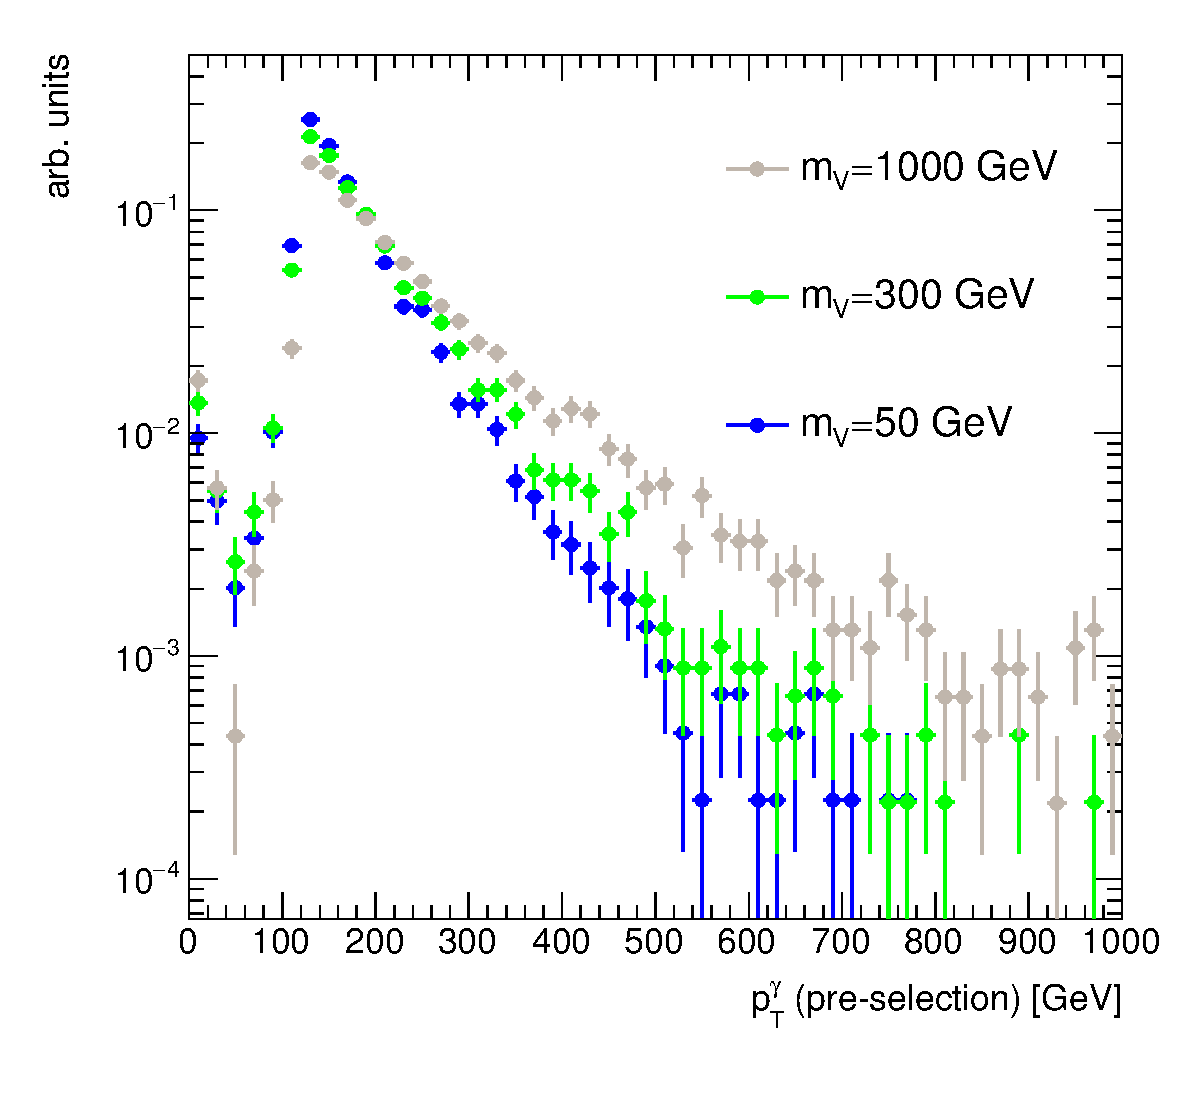
\includegraphics[width=0.45\textwidth]{figures/EW/ptGamma_filter120GeV_dmV_dm10GeV}
    }%TODO: add equivalent plot of MET to appendix
    \hfill
  \subfloat[Leading photon transverse momentum distribution for the photon+MET final state, 
  for different DM mass choices, with a mediator mass of 1 TeV.\label{fig:DMV_EW_gamma_pT}]{%
      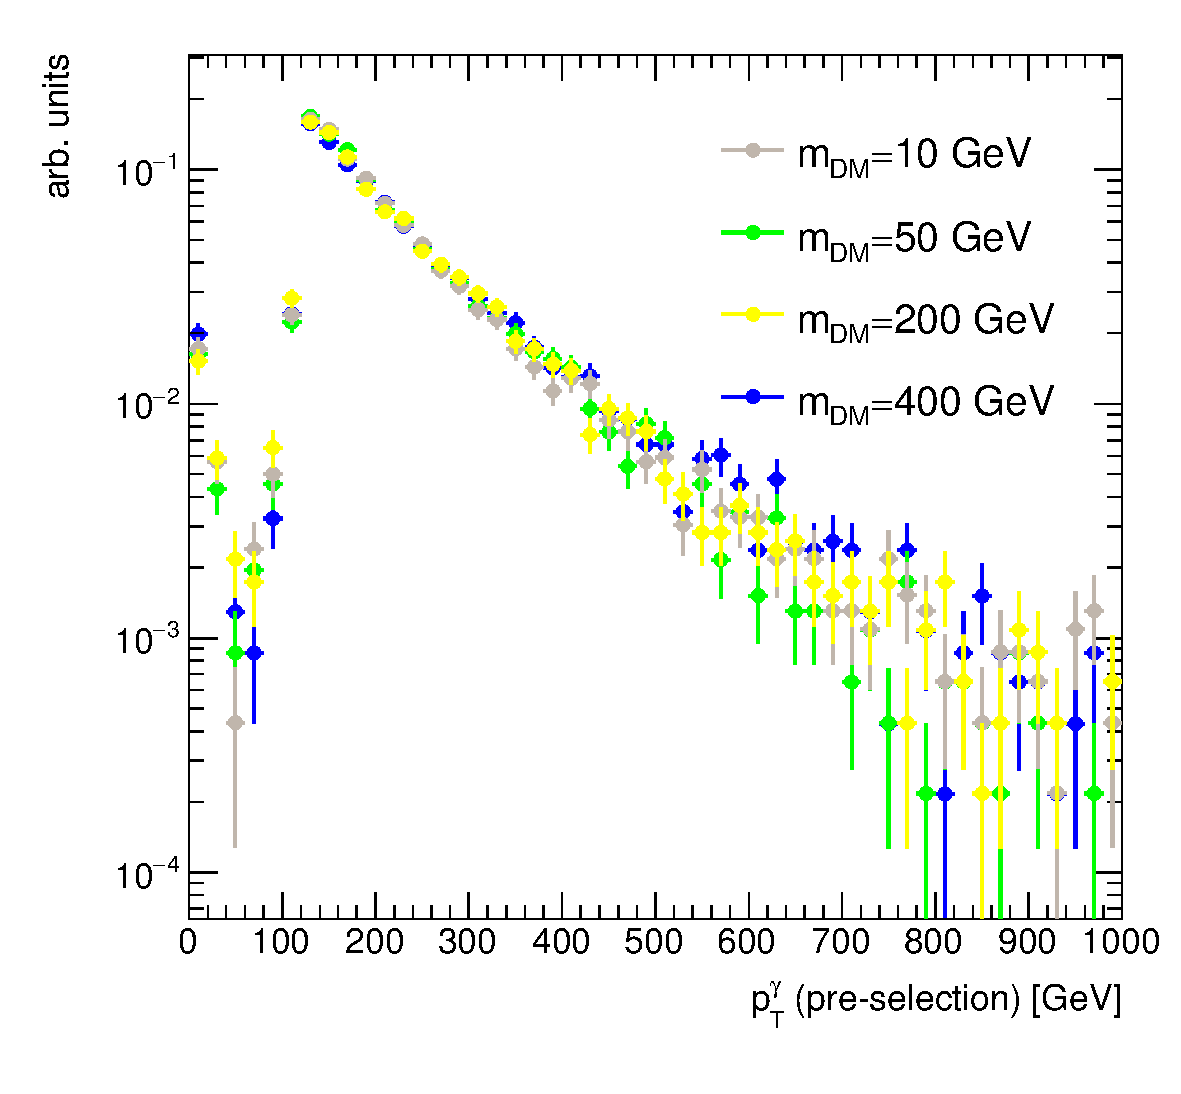
\includegraphics[width=0.45\textwidth]{figures/EW/ptGamma_filter120GeV_dmV_mV1000GeV}
    }%TODO: add equivalent plot of MET to appendix
    \hfill
  \subfloat[Missing transverse momentum distribution for the leptonic Z+MET final state.\label{fig:DMV_EW_Z_MET}]{%
      
\includegraphics[width=0.45\textwidth]{figures/llug}
    }    
  \subfloat[Transverse mass ($m_T$) for the leptonic W+MET final state.\label{fig:DMV_EW_Wlep_mT}]{%
      
\includegraphics[width=0.45\textwidth]{figures/gull}
    }
    \hfill
  \subfloat[Fat \textbf{[Insert algorithm]} jet mass ($m_T$) for the the hadronic W+MET final state.\label{fig:DMV_EW_Whad_jetMass}]{%
      
\includegraphics[width=0.45\textwidth]{figures/llug}
    }
    \caption{Kinematic distributions relevant for searches with W, Z and photons in the final state, 
    for the simplified model with a vector mediator exchanged in the $s-$channel.}
    \label{fig:DMV_EW_kinematics}
\end{figure}

\paragraph{Colored scalar mediator exchanged in the s-channel}

t-channel colored scalar, to be completed...

\paragraph{Model implementation}

These models are generated at leading order with MadGraph 2.2.2, and parameter
cards can be found on SVN \textbf{[TODO: Add SVN location]}.
The parton shower is done using Pythia 8, with a matching scale of... 
\textbf{[TODO: To be completed.]}

\newthought{EFT models with direct DM-boson couplings}

A complete list of effective operators with direct DM/boson couplings for
Dirac DM, up to dimension 7, can be found in~\cite{Cotta:2012nj}. 

Following the notation of~\cite{Carpenter:2012rg}, the dimension 5 benchmark models 
from this category have a Lagrangian that includes terms such as:

\begin{eqnarray}
\frac{m_W^2}{\Lambda_5^3} ~\bar{\chi} \chi ~W^{+ \mu} W^{-}_\mu
+ \frac{m_Z^2}{2 \Lambda_5^3} ~ \bar{\chi} \chi ~ Z^\mu Z_\mu ~.
\end{eqnarray}
 
where $m_Z$ and $m_W$ are the masses of the $Z$ and $W$ boson, $W^{\mu}$ and $Z^{\mu}$
are the fields of the gauge bosons, $\chi$ denote the Dark Matter fields 
and $\Lambda_5$ is the effective field theory scale. This operator 
induces signatures with MET in conjunction with Z and W bosons at tree level,
while at loop level it induces couplings to photon pairs and $Z \gamma$ through W loops. 
\textbf{[TODO: Ask Linda to explain this better than I did.]}.  
In these models, a clear relation exists between final states with photons, EW bosons
and Higgs boson. \textbf{[TODO: see if mono-Higgs studies exist for these operators, include them here]}.

The dimension 7 benchmark models include couplings to the kinetic
terms of the EW bosons ($F^{\mu\nu}_i$, with $F_i=1,2,3$ being the field strengths
of the SM $U(1)$ and $SU(2)$ gauge groups and $\tilde F^{\mu\nu}_i$ their dual tensors). 
The Lagrangian for the scalar coupling of DM and bosons include terms such as the following:

\begin{eqnarray}
\frac{1}{\Lambda_{7,S}^3} ~\bar{\chi} \chi ~ \sum_i k_i  F_i^{\mu \nu} F^i_{\mu \nu} + 
\frac{1}{\Lambda_{7,S}^3} ~\bar{\chi} \chi ~ \sum_i k_i  F_i^{\mu \nu} \tilde F^i_{\mu \nu}
\end{eqnarray}

The Lagrangian with pseudoscalar coupling includes the following terms:

\begin{eqnarray}
\frac{1}{\Lambda_{7,PS}^3} ~\bar{\chi} \gamma^5 \chi ~ \sum_i k_i  F_i^{\mu \nu} F^i_{\mu \nu} +
\frac{1}{\Lambda_{7,PS}^3} ~\bar{\chi} \gamma^5 \chi ~ \sum_i k_i  F_i^{\mu \nu} \tilde F^i_{\mu \nu}
\end{eqnarray}

The cut-off scales $\Lambda$ for the separate terms can be related to operators with different 
Lorentz structure from Ref.~\cite{Cotta:2012nj}. Given that they do not lead to 
substantial differences for collider searches as shown in Figure 2 of Ref.~\cite{Carpenter:2012rg}, 
they have been denoted as $\Lambda_{7,S}$ for the scalar case and  $\Lambda_{7,PS}$ for the pseudoscalar
case. 

The $k_i$ coefficients for the dimension 7 models are related to the couplings of DM to pairs of gauge 
bosons by gauge invariance: 

\begin{eqnarray}
% g_{gg}&=&\frac{k_3}{\Lambda_7^3} \\
g_{WW}&=&\frac{2k_2}{s_w^2 \Lambda_7^3} \\
g_{ZZ} &=& \frac{1}{4 s_w^2 \Lambda_7^3} \left(\frac{k_1 s_w^2}{c_w^2}+\frac{k_2 c_w^2}{s_w^2} \right) \\
g_{\gamma\gamma}&=&\frac{1}{4 c_w^2}\frac{k_1+k_2}{\Lambda_7^3} \\
g_{Z\gamma} &=& \frac{1}{2 s_w c_w \Lambda_7^3} \left(\frac{k_2}{s_w^2}-\frac{k_1}{c_w^2} \right)
\label{eq:prefactors}
\end{eqnarray}

where $s_w$ and $c_w$ are respectively the sine and cosine of the weak mixing angle. 

The coefficients $k_i$ determine the relative importance of each of the boson channels,
and their correlations. For example, for what concerns searches with W, Z and photons: 
\begin{itemize}
 \item $k_2$ alone controls the rate of the coupling to $W$ boson pairs;
 \item If $k_1 = k_2$ contributions from both $Z$ and $\gamma$ exchange appear;
 \item If $k_1 = c_w^2 / s_w^2 k_2$ the $\gamma$ exchange is negligible. 
\end{itemize}

The coefficients $k_1$ and $k_2$ are related to the coefficients $c_1$ and $c_2$ 
in the equivalent models of Ref.~\cite{Crivellin:2015wva} as $k_2 = s_w^2*c_2$ and $k_1=c_w^2 *c_1$.

\textbf{[TODO: Linda will possibly complete/correct this paragraph]} UV completions of 
such operators where the dominant signature is a single photon or EW boson are possible, 
for example through the exchange of a W' or a Z'. They are left as benchmarks for future searches as 
their implementation may require loop diagrams and need further studies beyond the timescale of this Forum. 

As shown in Fig.~\ref{fig:EW_EFT5_Zlep_MET}
kinematics of this model can be approximated by that of a simplified model including 
a high-mass scalar mediator exchanged in the s-channel. For this reason, 
the list of benchmark models with direct boson-DM couplings only includes dimension 7 operators. 
\textbf{[TODO: then we need to recommend the scalar mediator, 
but then the sensitivity is very poor wrt monojets - however, I still prefer
to generate a few (high-mass) simplified model points wrt an EFT if given the choice.]}

\begin{figure}
    
\includegraphics[width=0.6\textwidth]{figures/gull}
    \caption{Comparison of the missing transverse momentum for the simplified model
    where a scalar mediator is exchanged in the s-channel and the model including 
    a dimension-5 scalar contact operator, in the leptonic Z+MET final state}
    \label{fig:EW_EFT5_Zlep_MET}
\end{figure}

The kinematic distributions for dimension-7 scalar and pseudoscalar operators 
only shows small differences, as shown in Fig.~\ref{fig:EW_EFT5_gamma_MET}. 

\begin{figure}
    
\includegraphics[width=0.6\textwidth]{figures/llug}
    \caption{Comparison of the missing transverse momentum for the scalar and pseudoscalar
    operators with direct interaction between DM and photon, in the photon+MET final state}
    \label{fig:EW_EFT5_gamma_MET}
\end{figure}

Similarly, the differences in kinematics for the various signatures 
are negligible when changing the coefficients $k_1$ and $k_2$, as shown
in Figure~\ref{EFTD7_EW_kinematics}. Only the case $k_1=k_2=1$ is generated as benchmark; 
other cases are left for reinterpretation as they will only need a rescaling of the cross-sections
shown in Table~\ref{} \textbf{[TODO: add tables with cross sections]} for the various Dark Matter
mass points considered. 

\begin{figure}[h!]
  \centering  
  \subfloat[Missing transverse momentum distribution for the photon+MET final state.\label{fig:EFTD7_EW_gamma_MET}]{%
      
\includegraphics[width=0.45\textwidth]{figures/gull}
    }
    \hfill
  \subfloat[Missing transverse momentum distribution for the leptonic Z+MET final state.\label{fig:EFTD7_EW_Z_MET}]{%
      
\includegraphics[width=0.45\textwidth]{figures/llug}
    }    
  \subfloat[Transverse mass ($m_T$) for the leptonic W+MET final state.\label{fig:EFTD7_EW_Wlep_mT}]{%
      
\includegraphics[width=0.45\textwidth]{figures/gull}
    }
    \caption{Kinematic distributions relevant for searches with W, Z and photons in the final state, 
    for for the scalar and pseudoscalar operators representing direct interactions between DM and bosons.}
    \label{fig:EFTD7_EW_kinematics}
    
\end{figure}

Examples of relevant kinematic distributions for selected benchmark points are
shown in Fig.~\ref{fig:DMV_EW_kinematics}.

\begin{figure}[h!]
  \centering  
  \subfloat[Missing transverse momentum distribution for the photon+MET final state.\label{fig:DMV_EW_gamma_MET}]{%
      
\includegraphics[width=0.45\textwidth]{figures/gull}
    }
    \hfill
  \subfloat[Missing transverse momentum distribution for the leptonic Z+MET final state.\label{fig:DMV_EW_Z_MET}]{%
      
\includegraphics[width=0.45\textwidth]{figures/llug}
    }    
  \subfloat[Transverse mass ($m_T$) for the leptonic W+MET final state.\label{fig:DMV_EW_Wlep_mT}]{%
      
\includegraphics[width=0.45\textwidth]{figures/gull}
    }
    \hfill
  \subfloat[Fat \textbf{[Insert algorithm]} jet mass ($m_T$) for the the hadronic W+MET final state.\label{fig:DMV_EW_Whad_jetMass}]{%
      
\includegraphics[width=0.45\textwidth]{figures/llug}
    }
    \caption{Kinematic distributions relevant for searches with W, Z and photons in the final state, 
    for the simplified model with a vector mediator exchanged in the $s-$channel.}
    \label{fig:DMV_EW_kinematics}
\end{figure}

\paragraph{Specific simplified models}

Mono-Higgs, to be completed...

%%%

%%This is left here in case we want to recommend EFT benchmarks?
% \begin{description}
%  \item[Vector interaction with vector-vector couplings (D5)]. For both jet+MET and boson+MET searches, the kinematic of this operator corresponds to that of couplings that are vector-axial (D7), axial-axial (D8) and axial-vector (D6). In the case of W boson radiation, the three coupling scenarios $\xi=1,0,-1$ should be investigated. This operator populates the high MET
%  \item[Tensor interaction (D9)]. As shown in Figure \textbf{[CD: add picture from Andy]}, this operator populates a higher MET range with respect to the other operators chosen. 
%  \item[Scalar interaction (D1)]. This operator has the lowest cross-section and sensitivity at colliders in this final state, as DM production from light quarks via a scalar interaction is suppressed with respect to heavy quarks. However, it has the hardest MET spectrum of the EFT operators chosen, and results obtained using this operator as benchmark may be used for recasting signals with a similarly hard MET distribution.~\footnote{Q for Andy/M-E: ZZchichi max gamma: is it the same kinematics regardless of DM? See fig. 2 of ATLAS monoZ.}
% \end{description}
